	\section{Exercise 6: Floating Manipulation with Arm-Vehicle Coordination Scheme}
	\subsection{Adding the parallel arm-vehicle coordination scheme}
	\question
	Let us now see how the two different subsystems (arm and vehicle) can be
	properly coordinate. Introduce in the simulation a sinusoidal linear
	velocity disturbance acting on the vehicle (along a constant inertial
	x-y direction of your choice), and assume the actual vehicle velocity
	measurable. To do so, add a constant (in the inertial frame) velocity
	vector to the reference vehicle velocity before integrating it in the
	simulator.

	Goal: modify the control part to implement the parallel arm-vehicle
	coordination scheme. Observe that, even with a disturbance acting on the
	vehicle, the end-effector can stay in the required constant position.
	\begin{parts}
		\part{Which tasks did you introduce to implement the parallel
		coordination scheme?}
		\begin{solutionorbox}
			The TPIK is duplicated so that the second TPIK optimizes
			the arm velocities for the current reference vehicle
			velocities, from the first TPIK.

			In order to implement the parallel coordination scheme,
			the vehicle constrained velocity task is introduced at
			the top priority level of the second TPIK.
		\end{solutionorbox}

		\part{Show the plot of the position of the end-effector, showing
			that it is constant. Show also a plot of the velocities
		of the vehicle and of the arm.}

		\begin{solutionorbox}
			The plots are shown in Figure~\ref{fig:ex6_plots}.
		\end{solutionorbox}
		\begin{figure}[ht]
			\begin{subfigure}[b]{0.5\linewidth}
				\centering
				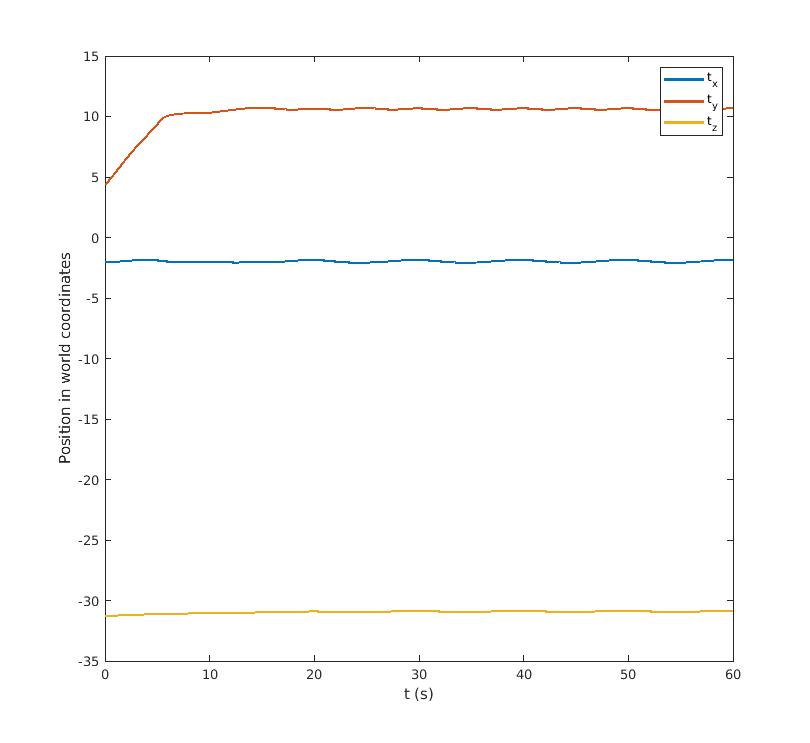
\includegraphics[width=\linewidth]{end_effector_position.jpg}
				\caption{End-effector position in world frame
				\cframe w}%
				\label{subfig:ee_position}
			\end{subfigure}%
			\begin{subfigure}[b]{0.5\linewidth}
				\centering
				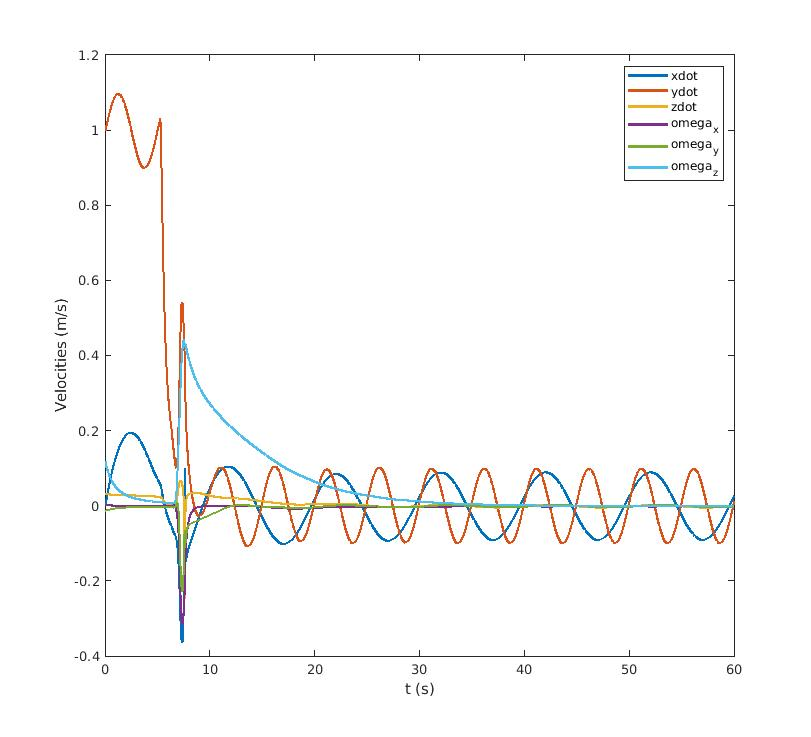
\includegraphics[width=\linewidth]{vehicle_velocities.jpg}
				\caption{Vehicle velocities}%
				\label{subfig:vehicle_velocities}
			\end{subfigure}
			\begin{subfigure}[b]{0.5\linewidth}
				\centering
				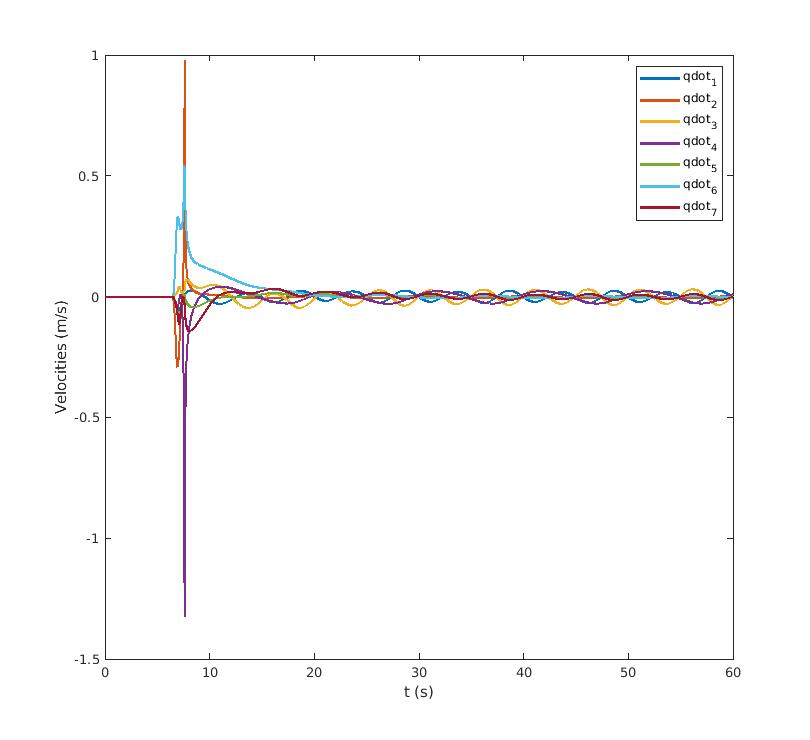
\includegraphics[width=\linewidth]{arm_velocities.jpg}
				\caption{Arm velocities}%
				\label{subfig:arm_velocities}
			\end{subfigure}

			\caption{End-effector position, vehicles and arm
			velocities with linear velocity disturbance along a $xy$
		direction}%
			\label{fig:ex6_plots}
		\end{figure}
		\label{part:ex6_2}
		\part{What happens if the sinusoidal disturbance becomes too big?
		Try increasing the saturation value of the end-effector task if it is too low.}

		\begin{solutionorbox}
			If the sinusoidal disturbance is too big, the
			end-effector position becomes variable, the arm tries to
			reach for the objective position when the vehicle comes
			near it.

			Despite increasing the saturation value, if the
			disturbance is too big, the TPIK cannot stabilise the
			end-effector position along the axis of the disturbance.

			The plots in question~\ref{part:ex6_2} have been updated
			in Figure~\ref{fig:ex6_plots_disturbed} to show the
			consequences of a big disturbance.
		\end{solutionorbox}

		\begin{figure}[ht]
			\begin{subfigure}[b]{0.5\linewidth}
				\centering
				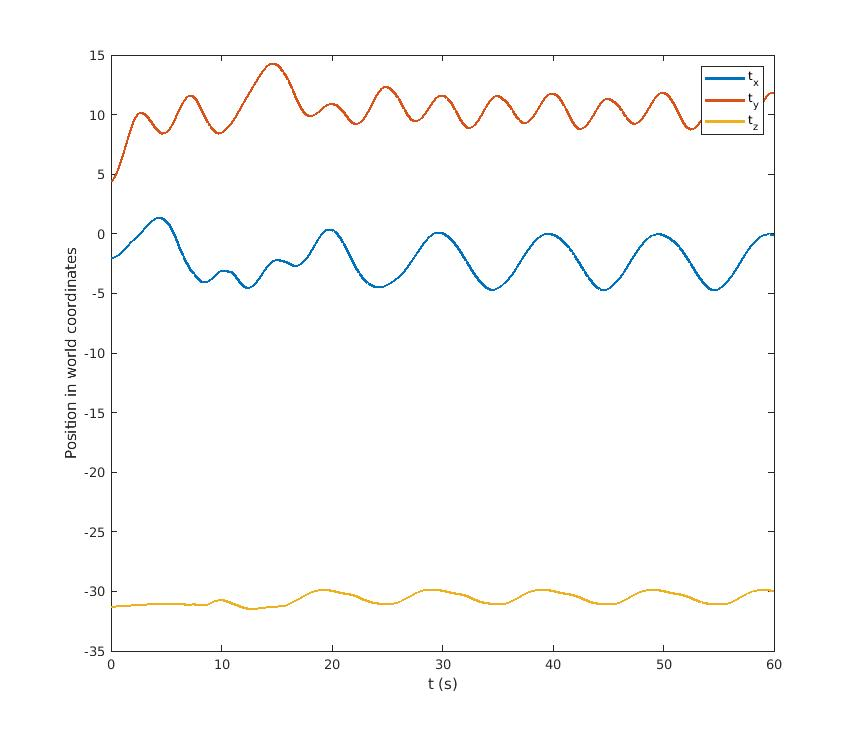
\includegraphics[width=\linewidth]{end_effector_position_disturbed.jpg}
				\caption{End-effector position in world frame
				\cframe w}%
				\label{subfig:ee_position_disturbed}
			\end{subfigure}%
			\begin{subfigure}[b]{0.5\linewidth}
				\centering
				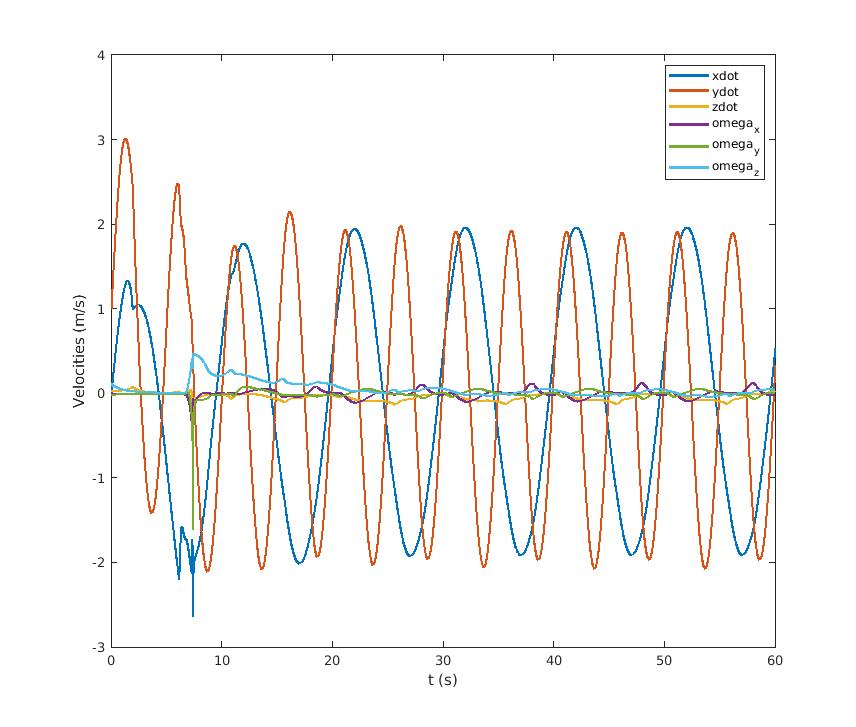
\includegraphics[width=\linewidth]{vehicle_velocities_disturbed.jpg}
				\caption{Vehicle velocities}%
				\label{subfig:vehicle_velocities_disturbed}
			\end{subfigure}
			\begin{subfigure}[b]{0.5\linewidth}
				\centering
				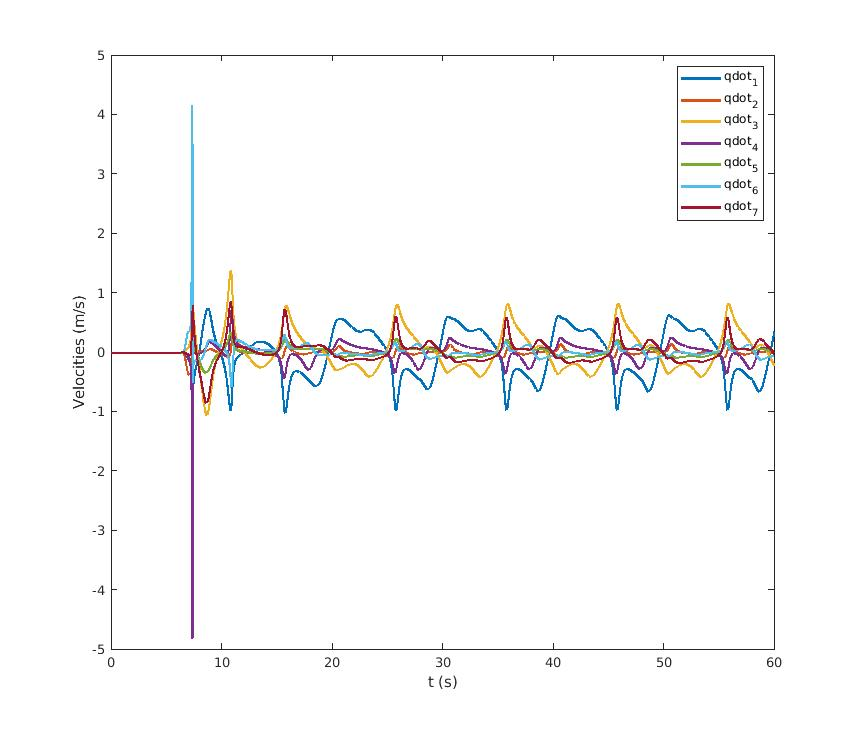
\includegraphics[width=\linewidth]{arm_velocities_disturbed.jpg}
				\caption{Arm velocities}%
				\label{subfig:arm_velocities_disturbed}
			\end{subfigure}

			\caption{End-effector position, vehicles and arm
			velocities with bigger linear velocity disturbance along
		a $xy$ direction}%
			\label{fig:ex6_plots_disturbed}
		\end{figure}

	\end{parts}

\end{questions}
